\documentclass[tikz,border=8pt]{standalone}
% Shared look for every TikZ diagram. Load with \input{../../tools/tikz-style.tex}
\usepackage[sfdefault]{roboto}
\usetikzlibrary{arrows.meta, positioning, shapes.geometric, calc, fit, backgrounds}
\definecolor{cblue}{HTML}{4C78A8}
\definecolor{corange}{HTML}{F58518}
\definecolor{cgreen}{HTML}{54A24B}
\definecolor{cred}{HTML}{E45756}
\definecolor{cpurple}{HTML}{B279A2}
\definecolor{cgrey}{HTML}{6B6B6B}
\tikzset{
  every picture/.style={font=\sffamily, line width=1.2pt},
  box/.style={draw=#1, fill=#1!12, rounded corners=4pt, align=center, inner sep=7pt, minimum height=1.1cm},
  box/.default=cgrey,
  arrow/.style={-{Stealth[length=3mm]}, draw=cgrey, line width=1.4pt},
  title/.style={font=\sffamily\bfseries\Large},
  note/.style={font=\sffamily\small, text=cgrey, align=center},
}
\AtBeginDocument{\hyphenpenalty=10000 \exhyphenpenalty=10000}

% Feedforward steering in two open stacks, read from their code on 2026-10-12.
% Apollo lat_based_lqr_controller/lat_controller.cc: steer = feedback (-K x, LQR) + ComputeFeedForward(curvature)
% + lead-lag augment; ComputeFeedForward = L kappa + kv v^2 kappa - K(0,2) (lr kappa - lf m v^2 kappa / (2 cr L)).
% Autoware autoware_mpc_lateral_controller: vehicle_model_bicycle_kinematics.cpp calculateReferenceInput
% u_ref = atan(wheelbase * curvature); mpc.cpp sets it to 0 below mpc_zero_ff_steer_deg = 0.5 deg.
\begin{document}
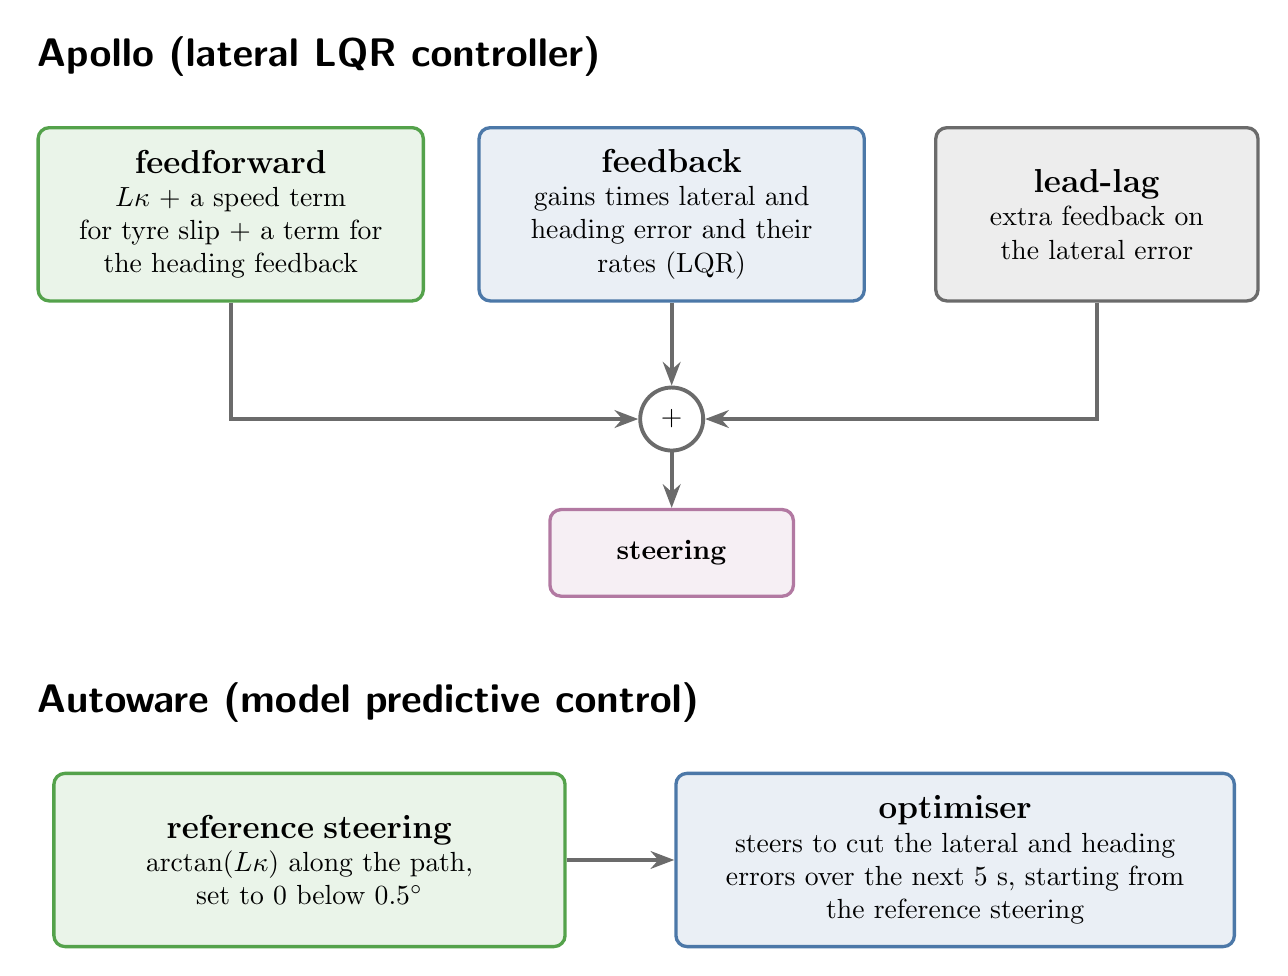
\begin{tikzpicture}[every node/.append style={font=\normalsize}, node distance=0.5cm,
  st/.style={box=#1, font=\normalsize, text width=4.4cm, minimum height=2.2cm}]
  \node[title, anchor=west] at (-2.6,2.0) {Apollo (lateral LQR controller)};
  \node[st=cgreen] (aff) at (0,0) {{\large\textbf{feedforward}}\\ $L\kappa$ + a speed term\\ for tyre slip + a term for\\ the heading feedback};
  \node[st=cblue] (afb) at (5.6,0) {{\large\textbf{feedback}}\\ gains times lateral and\\ heading error and their\\ rates (LQR)};
  \node[st=cgrey, text width=3.6cm] (aaug) at (11.0,0) {{\large\textbf{lead-lag}}\\ extra feedback on\\ the lateral error};
  \node[circle, draw=cgrey, line width=1.4pt, minimum size=0.8cm] (sum) at (5.6,-2.6) {$+$};
  \node[box=cpurple, text width=2.6cm] (st) at (5.6,-4.3) {\textbf{steering}};
  \draw[arrow] (aff.south) |- (sum.west); \draw[arrow] (afb) -- (sum); \draw[arrow] (aaug.south) |- (sum.east);
  \draw[arrow] (sum) -- (st);
  \node[title, anchor=west] at (-2.6,-6.2) {Autoware (model predictive control)};
  \node[st=cgreen, text width=6.0cm] (uref) at (1.0,-8.2) {{\large\textbf{reference steering}}\\ $\arctan(L\kappa)$ along the path,\\ set to 0 below $0.5^\circ$};
  \node[st=cblue, text width=6.6cm] (mpc) at (9.2,-8.2) {{\large\textbf{optimiser}}\\ steers to cut the lateral and heading\\ errors over the next 5 s, starting from\\ the reference steering};
  \draw[arrow] (uref) -- (mpc);
\end{tikzpicture}
\end{document}
